\documentclass{beamer}

\usetheme{Antibes}

% Loading preambulo
% PREAMBULO ====================================================================

% Packages ---------------------------------------------------------------------

% Package to Portuguese language
\usepackage[brazilian]{babel}
% Packages to Figures
\usepackage{graphicx}
\usepackage{tikz}
% Packages to math symbols and expressions
\usepackage{amsfonts, amssymb, amsmath}
% Packages to insert code
\usepackage{listings} 
\usepackage{verbatim}
% Package to justify text
\usepackage[document]{ragged2e}
% Package to manage the bibliography
\usepackage[backend=biber, style=numeric, sorting=none]{biblatex}
% Package to facilitate quotations
\usepackage{csquotes}
% Package to use multicols
\usepackage{multicol}
% Packages for url
%	The package libertinus already loads hyperref
%\usepackage[colorlinks=true]{hyperref}
% Font
%   Fira
%\usepackage[sfdefault, lf]{FiraSans}
%   Libertinus
\usepackage{libertinus}
\renewcommand*\familydefault{\sfdefault} %% Only if the base font of the document is to be sans serif
% Colors
\usepackage{xcolor}
\usepackage{colortbl}
% Table
\usepackage{tabularray}
% Fill line
\usepackage{xhfill}

% Configurations ---------------------------------------------------------------

\AtBeginSection{
    \begin{frame}{\secname}
        \tableofcontents[currentsection,hideallsubsections]
    \end{frame}
}

\AtBeginSubsection{
    \begin{frame}{\subsecname}
        \tableofcontents[currentsection,subsectionstyle=show/shaded/hide, subsubsectionstyle=hide]
    \end{frame}
}

\AtBeginSubsubsection{
    \begin{frame}{\subsubsecname}
        \tableofcontents[currentsection,subsectionstyle=show/shaded/hide,subsubsectionstyle=show/shaded/hide/hide]
    \end{frame}
}

% Numbering slides
\setbeamertemplate{footline}[frame number]{}

% Getting rid of bottom navigation bars
\setbeamertemplate{navigation symbols}{}

% Margins
\setbeamersize{text margin left=20pt, text margin right=20pt}

% Colors
\definecolor{burgundy}{RGB}{133,24,42}
\definecolor{bloodred}{RGB}{147,5,5}

\setbeamercolor{structure}{fg=burgundy}

\setbeamercolor*{palette primary}{use=structure,fg=white,bg=structure.fg}
%\setbeamercolor*{palette secondary}{use=structure,fg=white,bg=structure.fg!75!black}
%\setbeamercolor*{palette tertiary}{use=structure,fg=white,bg=structure.fg!50!black}
\setbeamercolor*{palette quaternary}{fg=white,bg=bloodred}

%	hyperref
\hypersetup{
	colorlinks=true,
	urlcolor=blue,
	breaklinks=true}

% New commands -----------------------------------------------------------------

\NewTblrTableCommand \aula{\SetCell{bg=green!60,fg=white}}
\NewTblrTableCommand \prova{\SetCell{bg=red!80,fg=white}}
\NewTblrTableCommand \feriado{\SetCell{bg=blue!50,fg=white}}

\newcommand{\esta}[1]{\textbf{\underline{#1}}}

% Title
\title[GP 02]{Gerência de Projetos}
% Subtitle
\subtitle{Princípios do Gerenciamento de Projetos - Parte 1}
% Author of the presentation
\author[E.J.R. Silva]{Evandro J.R. Silva}
% date of the presentation
\date{}

\begin{document}
    
\begin{frame}
    \titlepage
\end{frame}

\begin{frame}{Sumário}
    \tableofcontents
\end{frame}

%===============================================================================
% SECTION 1 ====================================================================
%===============================================================================
\section{Introdução}

\begin{frame}
	\justifying
	Os \textbf{princípios} de uma profissão \textbf{servem como diretrizes fundamentais para a estratégia}, \textbf{tomada de decisões} e \textbf{resolução de problemas}. Com frequência, \textbf{padrões} e \textbf{metodologias} profissionais \textbf{se baseiam em princípios}. Em algumas profissões, os princípios servem como leis ou regras e, assim, são prescritivos por natureza. Os \textbf{princípios do gerenciamento de projetos} \textbf{\alert{não} são de natureza prescritiva}. Pretendem apenas orientar o comportamento das pessoas envolvidas com projetos. Eles têm uma base ampla, então há muitas maneiras de as pessoas e as organizações manterem o alinhamento com os princípios.
\end{frame}

\begin{frame}
	\justifying
	Os princípios podem (embora não necessariamente) refletir a moral. Um código de ética está relacionado à moral. O código de ética de uma profissão pode ser adotado por uma pessoa ou profissão para definir expectativas de conduta moral. O \textit{Código de ética e conduta profissional}\footnote{Project Management Institute. 2006. \textit{PMI Code of Ethics and Professional Conduct}. Disponível em: \url{http://www.pmi.org/codeofethics}} tem em sua base os quatro valores identificados como os mais importantes para a comunidade de gerenciamento de projetos:
	\begin{itemize}
		\justifying
		\item Responsabilidade.
		\item Respeito.
		\item Equidade.
		\item Honestidade.
	\end{itemize}
\end{frame}

\begin{frame}
	\justifying
	Como os princípios do gerenciamento de projetos fornecem orientação, o \textbf{grau de aplicação} e a \textbf{maneira como são aplicados} são \textbf{influenciados} pelo \textbf{contexto da organização}, \textbf{do projeto}, \textbf{das entregas}, \textbf{da equipe do projeto}, \textbf{das partes interessadas} e de outros fatores. Internamente, os princípios são uniformes, ou seja, \textbf{nenhum princípio está em contradição com outro}. No entanto, na prática, pode haver situações em que os princípios se sobrepõem.
\end{frame}

\begin{frame}
	\begin{itemize}
		\item Os identificadores dos princípios estão aqui mencionados, sem nenhuma ponderação ou ordem:
			\begin{itemize}
				\justifying
				\item \textbf{Administração}: Seja um administrador diligente, respeitoso e atencioso.
				\item \textbf{Equipe}: Crie um ambiente colaborativo para a equipe do projeto.
				\item \textbf{Partes Interessadas}: Envolva-se de fato com as partes interessadas.
				\item \textbf{Valor}: Concentre-se no valor.
				\item \textbf{Pensamento Sistêmico}: Reconheça, avalie e reaja às interações do sistema.
				\item \textbf{Liderança}: Demonstre comportamentos de liderança.
				\item \textbf{\textit{Tailoring}}: Faça a adaptação de acordo com o contexto.
				\item \textbf{Qualidade}: Crie qualidade nos processos e nas entregas.
				\item \textbf{Complexidade}: Navegue pela complexidade.
				\item \textbf{Risco}: Otimize as respostas ao risco.
				\item \textbf{Capacidade de Adaptação e Resiliência}: Adote a capacidade de adaptação e resiliência.
				\item \textbf{Mudança}: Aceite a mudança para alcançar o futuro estado previsto.
			\end{itemize}
	\end{itemize}
\end{frame}

%===============================================================================
% SECTION 2 ====================================================================
%===============================================================================
\section{Princípios}

%-------------------------------------------------------------------------------
% SUBSECTION 2.1 ---------------------------------------------------------------
%-------------------------------------------------------------------------------
\subsection{Seja um administrador diligente, respeitoso e atencioso}

\begin{frame}{Seja um administrador diligente, respeitoso e atencioso}
	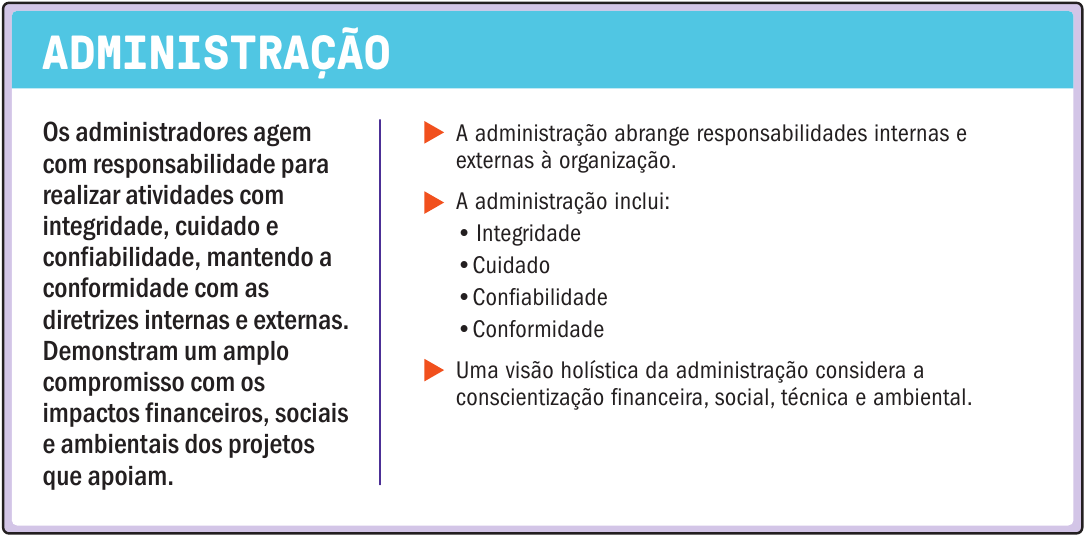
\includegraphics[width=\textwidth]{imagens/figura01.png}
\end{frame}

\begin{frame}{Seja um administrador diligente, respeitoso e atencioso}
	\begin{itemize}
		\justifying
		\item O objetivo da administração é alcançar os objetivos do projeto enquanto mantém a integridade, o cuidado, a confiabilidade e a conformidade.
		\item Administradores de projeto precisam praticar a gestão responsável tanto dentro quanto fora da organização. Eles devem ser diligentes, atenciosos e respeitosos com sua equipe, fornecedores, usuários finais, clientes e demais partes interessadas.
		\item Além disso, são responsáveis pelos impactos ambientais, sociais e financeiros do projeto.
	\end{itemize}
\end{frame}

\setbeamertemplate{background canvas}{%
	\tikz[remember picture,overlay] \node[opacity=0.15,inner sep=0pt] at (current page.center){
\includegraphics[width=\paperwidth,height=\paperheight]{imagens/Grace_Episcopal_Church,_Galveston,_Texas.jpg}};
}

\begin{frame}{Seja um administrador diligente, respeitoso e atencioso}
	\begin{itemize}
		\justifying
		\item Breve estudo de caso (\href{https://www.thepmoleader.com/blog/the-principles-of-being-a-good-steward-pmbok-3-1}{fonte})
			\begin{itemize}
				\justifying
				\item<1-> Jason Orloske ingressou no Conselho de uma igreja com mais de 1500 membros ativos.Como a igreja é 100\% financiada por doações, o Conselho precisava ser cuidadoso com as despesas, e também prestar contas.
				\item<2-> Para a prestação de contas foi implementada uma reunião trimestral (\textit{Quaterly Catch-UP}). Nesta reunião o Conselho compartilhava com a igreja questões financeiras, trabalhistas e também o andamento e planejamento de projetos. Por fim, a comunidade tinha um tempo para questionamentos e críticas.
				\item<3-> Em uma reunião foi apresentada a necessidade de manutenção da cozinha da igreja, o que resultaria em uma despesa considerável. Os membros da igreja (ou seja, os \textit{stakeholders}) compreenderam o problema e vários fizeram doação extra para cobrir os custos extras.
				\item<4> \textit{Feedback} de um dos membros: uma vez que o problema e os custos foram apresentados com antecedência, a igreja pôde interver proativamente, em vez de reativamente.
			\end{itemize}
	\end{itemize}
\end{frame}

\setbeamertemplate{background canvas}[default]

%\begin{frame}{Seja um administrador diligente, respeitoso e atencioso}
%	\begin{itemize}
%		\item Responsabilidades internas:
%			\begin{itemize}
%				\justifying
%				\item Trabalhar em alinhamento com a organização, seus objetivos, estra-tégia, visão, missão e sustentabilidade do seu valor em longo prazo;
%				\item Manter o compromisso e o engajamento respeitoso com os integrantes da equipe do projeto. Inclui também remuneração, acesso a oportunidades e tratamento justo;
%				\item Realizar supervisão diligente do recursos financeiros da organização, materiais e outros itens usados em um projeto;
%				\item Compreender o uso apropriado de autoridade, prestação de contas e responsabilidade, especialmente nas posições de liderança.
%			\end{itemize}
%	\end{itemize}
%\end{frame}
%
%\begin{frame}{Seja um administrador diligente, respeitoso e atencioso}
%	\begin{itemize}
%		\item Responsabilidades externas:
%		\begin{itemize}
%			\justifying
%			\item Sustentabilidade ambiental e uso de materiais e recursos naturais pela organização;
%			\item Relacionamento da organização com partes interessadas externas, como seus parceiros e canais;
%			\item Impacto da organização ou do projeto no mercado, na comunidade social e nas regiões em que atua;
%			\item Progresso do estado da prática em setores profissionais.
%		\end{itemize}
%	\end{itemize}
%\end{frame}
%
%\begin{frame}{Seja um administrador diligente, respeitoso e atencioso}
%	\begin{itemize}
%		\item Integridade
%			\begin{itemize}
%				\justifying
%				\item<1> Os administradores se comportam de maneira honesta e ética em todos os engajamentos e comunicações. 
%				\item<1> Ao mesmo tempo, devem desafiar os integrantes da equipe, colegas e outras partes interessadas a considerar suas palavras e ações; e ser empático, autorreflexivo e aberto a \textit{feedback}.
%			\end{itemize}
%		\item Cuidado
%			\begin{itemize}
%				\justifying
%				\item<2> Os administradores são depositários das questões organizacionais sob seu encargo e eles as supervisionam com diligência.
%				\item<2> O cuidado inclui a criação de um ambiente de trabalho transparente, canais de comunicação abertos e oportunidades para as partes interessadas levantarem questões sem culpa ou medo de retaliação.
%			\end{itemize}
%	\end{itemize}
%\end{frame}
%
%\begin{frame}{Seja um administrador diligente, respeitoso e atencioso}
%	\begin{itemize}
%		\item Confiabilidade
%			\begin{itemize}
%				\justifying
%				\item<1> Os administradores representam a si mesmos, seus papéis, sua equipe do projeto e sua autoridade com exatidão, dentro e fora da organização. 
%				\item<1> A confiabilidade também implica pessoas que identificam proativamente conflitos entre seus interesses pessoais e os dos clientes ou da sua organização.
%			\end{itemize}
%		\item Conformidade
%			\begin{itemize}
%				\justifying
%				\item<2> Os administradores cumprem leis, regras, regulamentos e exigências devidamente autorizados, dentro ou fora de suas organizações.
%				\item<2> Os administradores se esforçam para cumprir as diretrizes destinadas a protegê-los, à sua organização, às partes interessadas e ao público em geral.
%			\end{itemize}
%	\end{itemize}
%\end{frame}

%-------------------------------------------------------------------------------
% SUBSECTION 2.2 ---------------------------------------------------------------
%-------------------------------------------------------------------------------
\subsection{Crie um ambiente colaborativo para a equipe do projeto}

\begin{frame}{Crie um ambiente colaborativo para a equipe do projeto}
	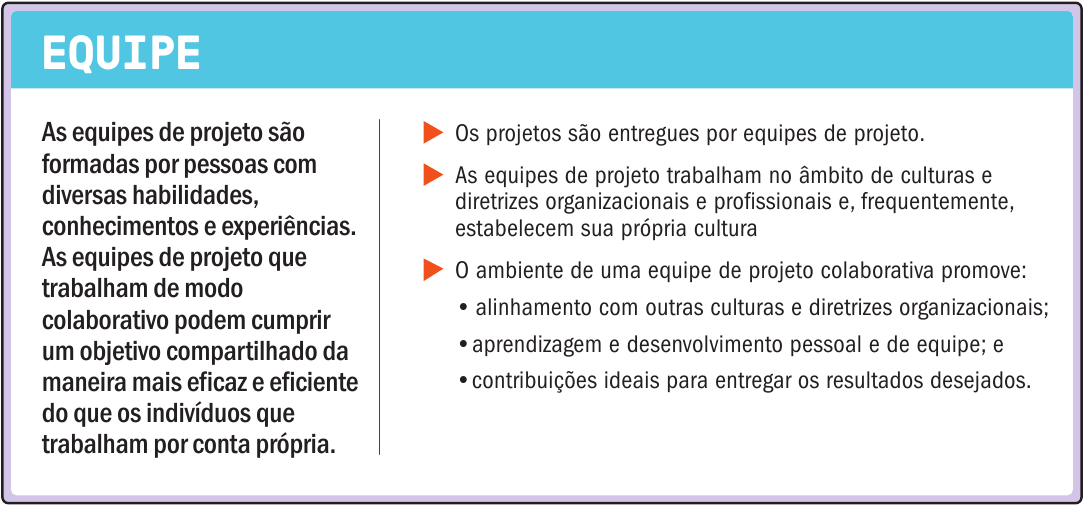
\includegraphics[width=\textwidth]{imagens/figura02.png}
\end{frame}

\begin{frame}{Crie um ambiente colaborativo para a equipe do projeto}
	\begin{itemize}
		\justifying
		\item<1,4> Membros de uma equipe possuem uma variedade de habilidades, expertise e experiências. Equipes que colaboram podem, portanto, alcançar um objetivo comum mais rápida e eficientemente do que pessoas trabalhando sozinhas. Logo, é muito importante fomentar um ambiente em que todos trabalham em prol do mesmo resultado.
		\item<2,4> Papéis e deveres precisam ser claramente definidos, e a equipe precisa trabalhar junta.
		\item<3,4> Além disso, um ambiente de equipe colaborativo promove o aprendizado e o crescimento tanto individual quanto coletivo, o alinhamento com outras culturas e políticas empresariais e as melhores contribuições possíveis para o alcance dos objetivos.
	\end{itemize}
\end{frame}

\setbeamertemplate{background canvas}{%
	\tikz[remember picture,overlay] \node[opacity=0.15,inner sep=0pt] at (current page.center){
\includegraphics[width=\paperwidth,height=\paperheight]{imagens/Google_Headquarters_Google_Logo_(52639793897).jpg}};
}

\begin{frame}{Crie um ambiente colaborativo para a equipe do projeto}
	\begin{itemize}
		\justifying
		\item Breve estudo de caso (\href{https://voltagecontrol.com/articles/successful-collaborative-leadership-in-action-case-studies-and-real-world-examples/}{fonte})
		\begin{itemize}
			\justifying
			\item<1-> O Google tem a política ``20\% time'', que consiste em permitir aos funcionários dedicarem um dia da semana para quaisquer projetos pessoais.
			\item<1-> Além disso, os escritórios foram planejados como espaços abertos, os quais encorajam interações espontâneas e multidisciplinares entre os funcionários.
			\item<2-> Resultados: criação de produtos de sucesso como \textbf{Google Suggest} (ferramenta de autocompletar), \textbf{AdSense}, \textbf{Google News}, \textbf{Google Translate} e o glorioso e saudoso \textbf{Orkut}.
		\end{itemize}
	\end{itemize}
\end{frame}

\setbeamertemplate{background canvas}[default]

%\begin{frame}{Crie um ambiente colaborativo para a equipe do projeto}
%	\begin{itemize}
%		\justifying
%		\item Criar um ambiente colaborativo para a equipe do projeto envolve vários fatores contribuintes como \alert<2>{acordos}, \alert<3>{estruturas} e \alert<4>{processos} da equipe.
%			\begin{itemize}
%				\justifying
%				\item<2> Representam um conjunto de parâmetros de comportamento e normas de trabalho estabelecidos pela equipe do projeto e mantidos pelo comprometimento pessoal e da equipe do projeto.
%				\item<3> São qualquer arranjo ou relação entre os elementos do trabalho do projeto e dos processos organizacionais. Podem ser baseadas em papéis, funções ou autoridade, ou ser definidas como externas ao projeto.
%				\item<4> Permitem a conclusão de tarefas e as atribuições de trabalho.
%			\end{itemize}
%		\item Esses fatores apoiam a cultura que permite o trabalho conjunto das pessoas e fornece efeitos sinérgicos a partir das interações.
%	\end{itemize}
%\end{frame}
%
%\begin{frame}{Crie um ambiente colaborativo para a equipe do projeto}
%	\begin{itemize}
%		\justifying
%		\item Criar um ambiente colaborativo para a equipe do projeto envolve vários fatores contribuintes como \alert<2>{acordos}, \alert<3>{estruturas} e \alert<4>{processos} da equipe.
%		\begin{itemize}
%			\justifying
%			\item<2> Representam um conjunto de parâmetros de comportamento e normas de trabalho estabelecidos pela equipe do projeto e mantidos pelo comprometimento pessoal e da equipe do projeto.
%			\item<3> São qualquer arranjo ou relação entre os elementos do trabalho do projeto e dos processos organizacionais. Podem ser baseadas em papéis, funções ou autoridade, ou ser definidas como externas ao projeto.
%			\item<4> Permitem a conclusão de tarefas e as atribuições de trabalho.
%		\end{itemize}
%		\item Esses fatores apoiam a cultura que permite o trabalho conjunto das pessoas e fornece efeitos sinérgicos a partir das interações.
%	\end{itemize}
%\end{frame}

%-------------------------------------------------------------------------------
% SUBSECTION 2.3 ---------------------------------------------------------------
%-------------------------------------------------------------------------------
\subsection{Envolva-se de fato com as partes interessadas}

\begin{frame}{Envolva-se de fato com as partes interessadas}
	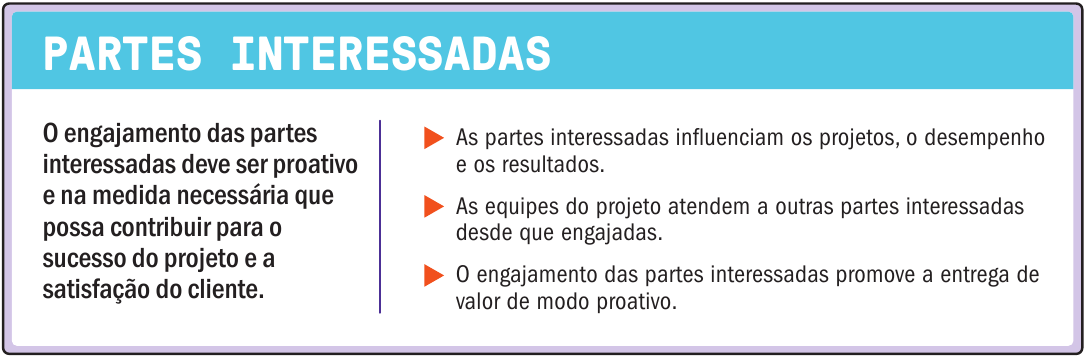
\includegraphics[width=\textwidth]{imagens/figura03.png}
\end{frame}

\begin{frame}{Envolva-se de fato com as partes interessadas}
	\begin{itemize}
		\justifying
		\item As partes interessadas (\textit{stakeholders}) têm um impacto significativo no resultado do projeto. Portanto, é essencial incluí-las proativamente e na medida necessária para apoiar o sucesso do projeto e a satisfação do cliente.
		\item A comunicação eficaz é necessária para envolver as partes interessadas de forma eficiente. Isso também inclui a escolha de estratégias de comunicação, como ``como'', ``quando'' e ``com que frequência''.
		\item O envolvimento das partes interessadas ajuda a evitar seus potenciais impactos negativos e a aumentar os impactos positivos no projeto.
	\end{itemize}
\end{frame}

\setbeamertemplate{background canvas}{%
	\tikz[remember picture,overlay] \node[opacity=0.15,inner sep=0pt] at (current page.center){
\includegraphics[width=\paperwidth,height=\paperheight]{imagens/Australia_Victoria_relief_location_map.jpg}};
}

\begin{frame}{Envolva-se de fato com as partes interessadas}
	\begin{itemize}
		\justifying
		\item Breve estudo de caso (\href{https://quicker.com.au/community-engagement/stakeholder-management-examples-real-world-use-cases-best-practices/}{fonte})
		\begin{itemize}
			\justifying
			\item<1-> Um Conselho Local no Estado Victoria, da Austrália, lançou um projeto de revitalização da paisagem urbana. Consultas iniciais, por meio de assembleias públicas, indicaram um forte interesse público, misturado com preocupações acerca de acessibilidade e estacionamento.
			\item<2-> Usando uma plataforma de engajamento o Conselho mapeou os \textit{stakeholders}, os segmentou de acordo com sua influência e importância, e depois usou de pesquisas direcionadas, fóruns e enquetes rápidas para envolver moradores, empresas e autoridades.
			\item<3-> Resultado: menor oposição, maior apoio da comunidade e maior transparência política.
		\end{itemize}
	\end{itemize}
\end{frame}

\setbeamertemplate{background canvas}[default]

%-------------------------------------------------------------------------------
% SUBSECTION 2.4 ---------------------------------------------------------------
%-------------------------------------------------------------------------------
\subsection{Enfoque no valor}

\begin{frame}{Enfoque no valor}
	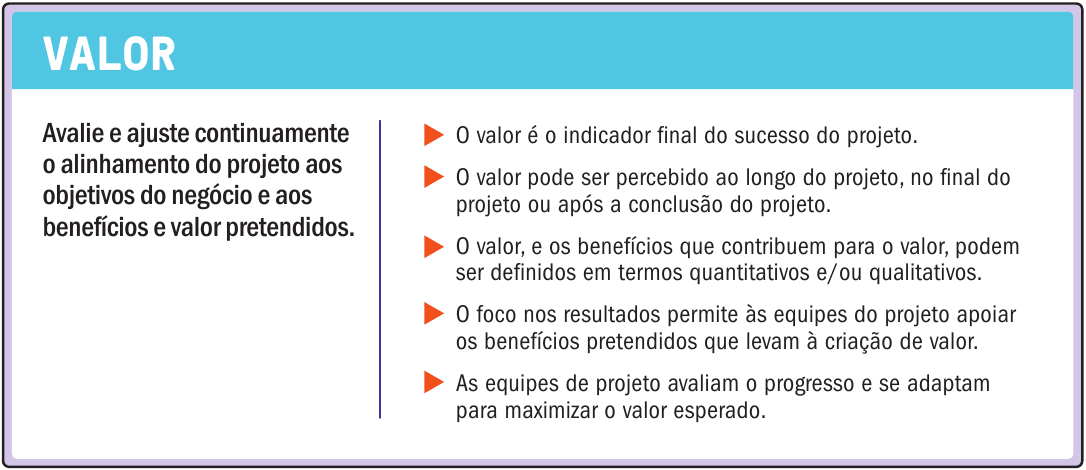
\includegraphics[width=\textwidth]{imagens/figura04.png}
\end{frame}

\begin{frame}{Enfoque no valor}
	\begin{itemize}
		\justifying
		\item O indicador final do sucesso de um projeto é o valor. Ele pode ser alcançado em qualquer ponto do projeto, mesmo após sua conclusão.
		\item Os membros da equipe devem definir o propósito do projeto e se esforçar para atender a uma necessidade específica do negócio, agregando valor ao projeto.
		\item Alinhar as partes interessadas com a visão é essencial para a geração de valor. As equipes devem se preocupar mais com o resultado desejado do que com as entregas. Além disso, o valor varia entre diferentes projetos e negócios.
	\end{itemize}
\end{frame}

\setbeamertemplate{background canvas}{%
	\tikz[remember picture,overlay] \node[opacity=0.15,inner sep=0pt] at (current page.center){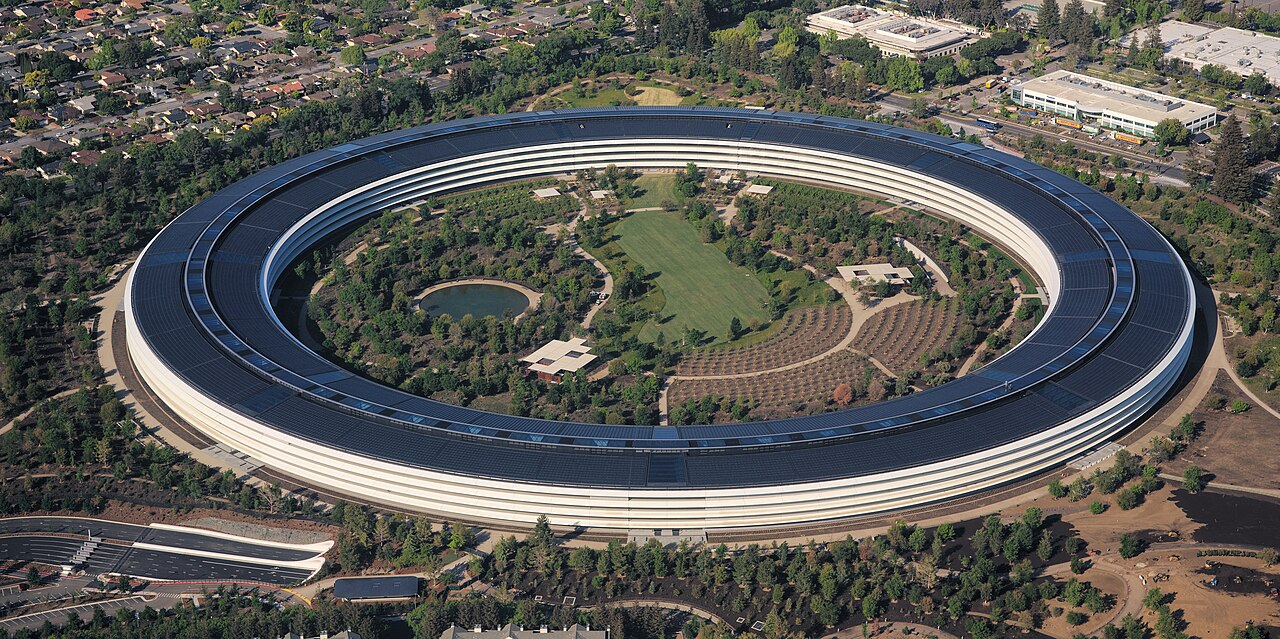
\includegraphics[width=\paperwidth,height=\paperheight]{imagens/Aerial_view_of_Apple_Park_dllu_(cropped).jpg}};
}

\begin{frame}{Enfoque no valor}
	\begin{itemize}
		\justifying
		\item Breve estudo de caso (\href{https://www.macworld.com/article/219225/steve-jobss-seven-key-decisions.html}{fonte})
		\begin{itemize}
			\justifying
			\item<1-> Antes da volta de Steve Jobs em 1997, a Apple fabricava dezenas de modelos diferentes de computadores desktop, laptops e servidores Macintosh em uma variedade impressionante de opções. A empresa também produzia linhas de impressoras, câmeras digitais e outros itens auxiliares, dos quais poucos davam lucro. Eram mais de 350 produtos.
			\item<2-> Jobs cortou mais de 70\% dos produtos de hardware e software, sendo o Newton PDA um dos cortes mais famosos. Foi nesse período que ocorreu uma das histórias mais famosas: Jobs desenhou num quadro branco uma cruz simples organizando os produtos a serem focados, divididos por nicho: Consumidor/Profissional e Desktop/Portátil.
			\item<3-> Resultado: iMac voltou a ser relevante (1998); iPod redefiniu o consumo de música (2001); iPhone revolucionou o mercado de celulares (2007); iPad criou/ressuscitou uma nova categoria de produtos (2010).
			\item<4> Steve Jobs explicando os cortes da Apple no Worldwide Developer Conference em 1997: \href{https://www.youtube.com/watch?v=oeqPrUmVz-o}{vídeo}.
		\end{itemize}
	\end{itemize}
\end{frame}

\setbeamertemplate{background canvas}[default]

%-------------------------------------------------------------------------------
% SUBSECTION 2.5 ---------------------------------------------------------------
%-------------------------------------------------------------------------------
\subsection{Reconheça, avalie e reaja às interações do sistema}

\begin{frame}{Reconheça, avalie e reaja às interações do sistema}
	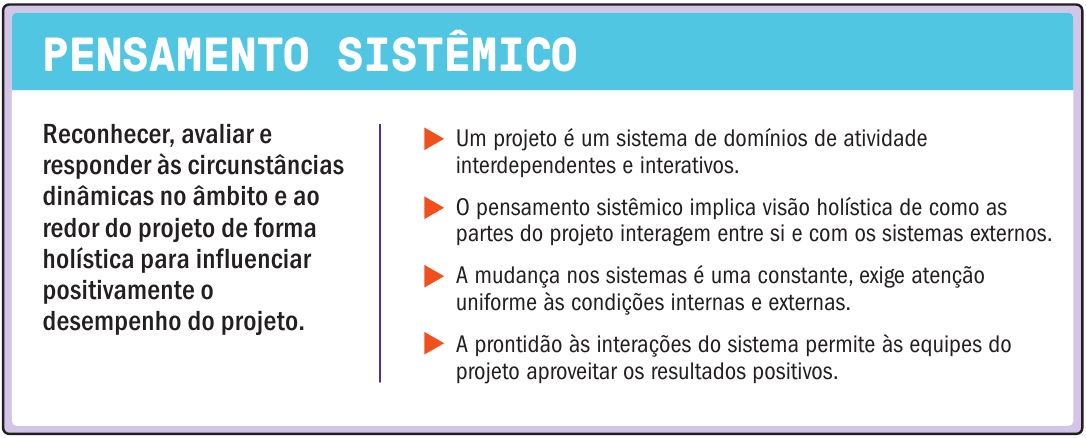
\includegraphics[width=\textwidth]{imagens/figura05.png}
\end{frame}

\begin{frame}{Reconheça, avalie e reaja às interações do sistema}
	\begin{itemize}
		\justifying
		\item O PMBOK 7 considera um projeto como um sistema composto por indivíduos, processos, tecnologia e outros componentes internos e externos interconectados.
		\item Portanto, os gerentes de projeto precisam lidar com os efeitos das mudanças nas circunstâncias internas e externas e adotar uma mentalidade holística.
		\item Além disso, os sistemas são dinâmicos, o que significa que tanto os fatores internos quanto os externos precisam ser monitorados continuamente.
		\item As equipes de projeto devem, portanto, estar atentas às interações do sistema para que possam aproveitar os resultados favoráveis.
	\end{itemize}
\end{frame}

\setbeamertemplate{background canvas}{%
	\tikz[remember picture,overlay] \node[opacity=0.15,inner sep=0pt] at (current page.center){
\includegraphics[width=\paperwidth,height=\paperheight]{imagens/Hospital.png}};
}

\begin{frame}{Reconheça, avalie e reaja às interações do sistema}
	\begin{itemize}
		\justifying
		\item Breve estudo de caso (\href{https://strategic-engineering.co/blog/concepts/systems-thinking/}{fonte})
		\begin{itemize}
			\justifying
			\item<1-> Em um hospital, o uso de mapeamento de fluxos (\textit{stocks} e \textit{flows}) identificou um gargalo no laboratório \textit{downstream} que causava longas esperas no pronto-socorro.
			\item<2-> Adicionando apenas um técnico noturno, o tempo médio de espera foi reduzido em 25\%, considerando interações entre admissões, descargas e recursos externos.
		\end{itemize}
	\end{itemize}
\end{frame}

\setbeamertemplate{background canvas}[default]

%-------------------------------------------------------------------------------
% SUBSECTION 2.6 ---------------------------------------------------------------
%-------------------------------------------------------------------------------
\subsection{Demonstre comportamentos de liderança}

\begin{frame}{Demonstre comportamentos de liderança}
	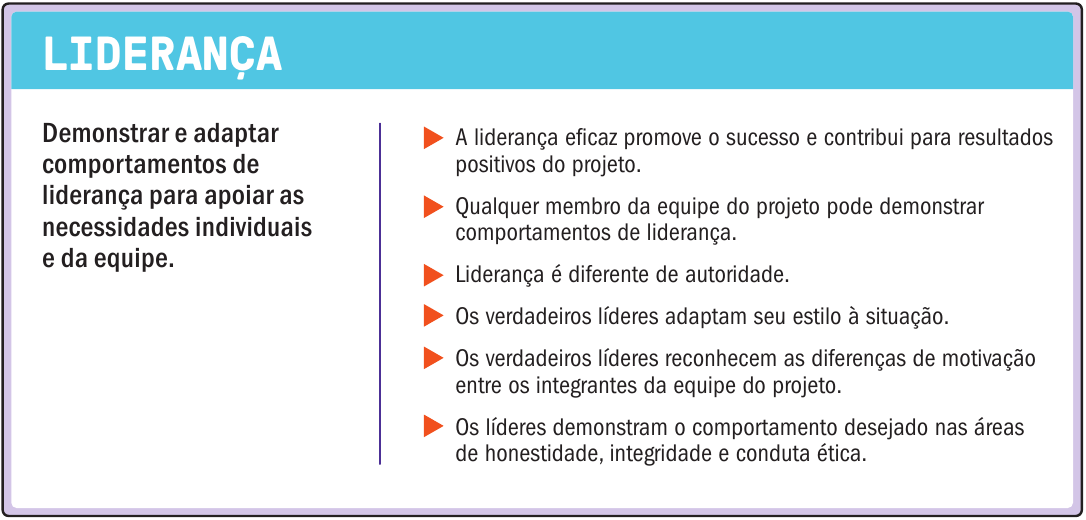
\includegraphics[width=\textwidth]{imagens/figura06.png}
\end{frame}

\begin{frame}{Demonstre comportamentos de liderança}
	\begin{itemize}
		\justifying
		\item O sucesso e os resultados favoráveis de um projeto são impulsionados por uma liderança eficaz.
		\item Profissionais que aspiram a ser grandes líderes devem fomentar um ambiente rico em inspiração, motivação, entusiasmo, empatia e apoio. Devem estar atentos às variações de motivação entre os membros da equipe do projeto.
		\item Além disso, devem demonstrar a conduta desejada em termos de ética, honestidade e integridade.
		\item Sob esse tipo de liderança, os membros da equipe podem trabalhar melhor e alcançar os resultados pretendidos.
	\end{itemize}
\end{frame}

\setbeamertemplate{background canvas}{%
	\tikz[remember picture,overlay] \node[opacity=0.15,inner sep=0pt] at (current page.center){
\includegraphics[width=\paperwidth]{imagens/The_new_logo_of_Johnson_&_Johnson.png}};
}

\begin{frame}{Demonstre comportamentos de liderança}
	\begin{itemize}
		\justifying
		\item Breve estudo de caso (\href{https://en.wikipedia.org/wiki/Chicago_Tylenol_murders}{fonte})
		\begin{itemize}
			\justifying
			\item<1-> Em 1982 aconteceu a crise de contaminação do Tylenol, quando sete pessoas em Chicago morreram após ingerir cápsulas de Tylenol Extra Forte adulteradas com cianeto.
			\item<2-> A Johnson \& Johnson demonstrou liderança adaptável ao recalls imediato de 31 milhões de frascos, priorizando ética e integridade sobre custos (US\$ 100 milhões).
			\item<3-> O CEO James Burke motivou a equipe com transparência, empatia e foco em segurança pública, adaptando o estilo à situação de crise. Isso não só restaurou a confiança dos \textit{stakeholders}, mas também aumentou a participação de mercado, ilustrando como comportamentos de liderança inspiram equipes e diferenciam autoridade de influência real.
		\end{itemize}
	\end{itemize}
\end{frame}

\setbeamertemplate{background canvas}[default]

%===============================================================================
% SECTION 3 ====================================================================
%===============================================================================
\section{Atividade}

\begin{frame}{Atividade}
	\begin{itemize}
		\justifying
		\item Dividam-se em 6 grupos.
		\item O grupo deverá analisar os problemas disponíveis nos próximos slides e, para cada problema:
			\begin{itemize}
				\justifying
				\item Identificar qual princípio está sendo negligenciado.
				\item Identificar/sumarizar o problema central.
				\item Propor ações corretivas.
				\item Identificar riscos financeiros, reputacionais e humanos.
				\item Avaliar consequências das decisões.
			\end{itemize}
		\item Os grupos terão um tempo para discutir sobre cada problema e, ao fim, vamos debater sobre as respostas.
	\end{itemize}
\end{frame}

\begin{frame}{Atividade}
	\begin{itemize}
		\justifying
		\item \textbf{Problema 1}
			\begin{itemize}
				\justifying
				\item Startup desenvolve plataforma adaptativa para ensino técnico. 
				\item Os investidores exigem:
					\begin{itemize}
						\justifying
						\item MVP funcional em 90 dias.
						\item Métricas mínimas de engajamento.
					\end{itemize}
				\item Após 60 dias:
					\begin{itemize}
						\justifying
						\item Desenvolvedor sênior pede desligamento.
						\item UX designer relata \textit{burnout}.
						\item Discussões se tornam frequentes.
						\item Entregas começam a atrasar.
					\end{itemize}
%				\item O gerente do projeto tem duas opções:
%					\begin{itemize}
%						\justifying
%						\item Aumentar pressão e controle.
%						\item Redefinir estratégia e postura.
%					\end{itemize}
			\end{itemize}
	\end{itemize}
\end{frame}

\begin{frame}{Atividade}
	\begin{itemize}
		\justifying
		\item \textbf{Problema 2}
		\begin{itemize}
			\justifying
			\item Prefeitura implementa sistema de transporte integrado com:
				\begin{itemize}
					\item Monitoramento por GPS da frota.
					\item Aplicativo de previsão de chegada.
					\item Centro de controle.
					\item Integração com dados meteorológicos.
					\item Portal de transparência pública.
				\end{itemize}
			\item Durante o desenvolvimento:
				\begin{itemize}
					\item Mudança de prefeito altera prioridades.
					\item Lei federal sobre proteção de dados impõe novas regras.
					\item Sindicato de motoristas protesta contra monitoramento.
					\item Chuvas intensas afetam infraestrutura.
				\end{itemize}
			\item Cada evento impacta múltiplos subsistemas.
		\end{itemize}
	\end{itemize}
\end{frame}

\begin{frame}{Atividade}
	\begin{itemize}
		\justifying
		\item \textbf{Problema 3}
		\begin{itemize}
			\justifying
			\item Indústria metalúrgica com 320 funcionários decide substituir sistema legado por ERP moderno.
			\item Objetivos estratégicos declarados:
				\begin{itemize}
					\item Redução de desperdício.
					\item Melhor controle de estoque.
					\item Aumento de previsibilidade na produção.
				\end{itemize}
			\item Durante as reuniões iniciais:
				\begin{itemize}
					\item Diretoria solicita dezenas de relatórios personalizados.
					\item Cada gerente pede \textit{dashboards} específicos.
					\item Equipe técnica desenvolve tudo conforme solicitado.
				\end{itemize}
			\item Projeto é concluído no prazo e orçamento.
			\item Após 6 meses:
				\begin{itemize}
					\justifying
					\item Operadores evitam usar o sistema.
					\item Dados continuam sendo controlados em planilhas paralelas.
					\item ROI não é atingido.
				\end{itemize}
		\end{itemize}
	\end{itemize}
\end{frame}

\begin{frame}{Atividade}
	\begin{itemize}
		\justifying
		\item \textbf{Problema 4}
			\begin{itemize}
				\justifying
				\item Uma universidade privada adquire um terreno próximo a área residencial para expandir cursos de engenharia.
				\item Projeto inclui:
					\begin{itemize}
						\item 4 novos blocos.
						\item Laboratórios.
						\item Estacionamento para 800 veículos.
					\end{itemize}
				\item \textit{Stakeholders} identificados inicialmente:
					\begin{itemize}
						\item Conselho administrativo.
						\item Investidores.
						\item Corpo docente.
					\end{itemize}
				\item Moradores da região não foram formalmente mapeados.
				\item Após início das obras:
					\begin{itemize}
						\justifying
						\item Associação de moradores entra com ação judicial.
						\item Alegam aumento de tráfego, ruído e desvalorização imobiliária.
						\item Prefeitura exige novo estudo de impacto urbano.
					\end{itemize}
				\item Obra é embargada temporariamente.
			\end{itemize}
	\end{itemize}
\end{frame}

\begin{frame}{Atividade}
	\begin{itemize}
		\justifying
		\item \textbf{Problema 5}
			\begin{itemize}
				\justifying
				\item Uma \textit{healthtech} foi contratada pelo governo estadual para implantar telemedicina em municípios isolados.
				\item Equipe do projeto:
					\begin{itemize}
						\item Desenvolvedores backend (São Paulo).
						\item Médicos especialistas (Manaus).
						\item Equipe de UX.
						\item Consultor regulatório.
						\item Representantes de postos de saúde locais.
					\end{itemize}
				\item Problemas iniciais:
					\begin{itemize}
						\item Desenvolvedores priorizam performance.
						\item Médicos reclamam da usabilidade clínica.
						\item Consultor regulatório alerta sobre LGPD.
						\item Profissionais do interior dizem que a internet é instável.
					\end{itemize}
				\item Cada grupo trabalha isoladamente. Após 2 meses:
					\begin{itemize}
						\item Retrabalho elevado.
						\item Conflitos em reuniões.
						\item Atraso acumulado de 20\%.
					\end{itemize}
			\end{itemize}
	\end{itemize}
\end{frame}

\begin{frame}{Atividade}
	\begin{itemize}
		\justifying
		\item \textbf{Problema 6}
			\begin{itemize}
				\justifying
				\item Uma universidade federal com 18 mil alunos enfrenta instabilidade no sistema de matrícula há anos. A cada semestre:
					\begin{itemize}
						\item Servidores caem nas primeiras horas.
						\item Alunos perdem disciplinas.
						\item Há pressão política da reitoria.
					\end{itemize}
				\item Foi aprovado um projeto de R\$ 2 milhões para modernização da infraestrutura e desenvolvimento de novo sistema. O contrato prevê SLA (Acordo de Nível de Serviço) mínimo, mas não especifica detalhes técnicos de redundância.
				\item Durante a execução:
					\begin{itemize}
						\justifying
						\item O gerente da empresa fornecedora identifica que pode economizar R\$ 300 mil substituindo o cluster redundante por solução simplificada.
						\item A probabilidade de falha aumenta apenas em períodos de pico.
						\item O lucro do fornecedor aumentaria significativamente.
					\end{itemize}
			\end{itemize}
	\end{itemize}
\end{frame}

%===============================================================================
% FIM ==========================================================================
%===============================================================================

\begin{frame}
    \centering
    \Large
    FIM
\end{frame}
    
\end{document}
